\chapter{PyZX: ZX-Calculus Using Python}
\label{ch:pyzx}

% \section{So, What is PyZX?}
Now that we have a basic understanding about ZX-Calculus, we can now take our knowledge a step further into a more computational approach. Since we have already installed PyZX as a package in the previous chapter, we will dive more into quantum circuits and how this library works.

\large{PyZX} is a Python-based library designed with the purpose of reasoning with large {quantum circuits} and {ZX-diagrams}. Luckily for us, it is  an open-source resource -- and completely free! With PyZX, we can efficiently rewrite ZX-diagrams using some simplification strategies. And don't think these "strategies" are not that important -- they are so powerful that they are able to perform highly effective T-count optimization and even to verify correctness of optimised circuits. 

If you think that's {not enough}, PyZX also offers diverse ways to visualise circuits and ZX-diagrams. With this tool, we will be able to present circuits in QC, QASM and Quipper formats, and it can also convert ZX-diagrams into TikZ diagrams. In short, PyZX is a really powerful tool for circuit optimization; for example, to optimize multiple circuits or combining these with other external procedures. 

\section{Overview}
We will now specify the main features of PyZX and how you can implement them. The objective of this section is not to give a detailed tutorial, but rather a brief tour of what PyZX can do. If you are interested in deepening the concepts presented, that's completely fine! We will provide resources for further study in the last section of the chapter. 

\subsection{ZX-diagrams and circuits}
There are two main data-structures present in PyZX: \texttt{Circuits} and \texttt{Graphs}. A \texttt{Circuit} is a wrapper around a list of gates, while a \texttt{Graph} represents a ZX-diagram.

\subsubsection{\texttt{Circuit} class}
To be more precise, the \texttt{Circuit} class is the entry-point for importing and exporting circuits to and from PyZX. There are also multiple ways to implement optimization schemes that directly act onto the \texttt{Circuit} (however, we will explain that in the "Circuit Optimisation" chapter). So, to wrap the definition up, a \texttt{Circuit} is a list of \texttt{Gates} that can be converted into various representations, like ZX-diagrams or the QASM format. The way to import a circuit into PyZX is the following:
\begin{minted}{python}
circuit = zx.Circuit.load("path/to/circuit.extension")
\end{minted}

With this, PyZX will automatically try to figure out in which format the circuit is represented! There is also a way to generate random circuits:
\begin{minted}{python}
>>> circuit = zx.generate.CNOT_HAD_PHASE_circuit(qubits=10,depth=20,clifford=True)
\end{minted}

Also, if you use \texttt{zx.draw}, a matplotlib figure would be returned instead. 

\begin{figure}[H]
        \centering
        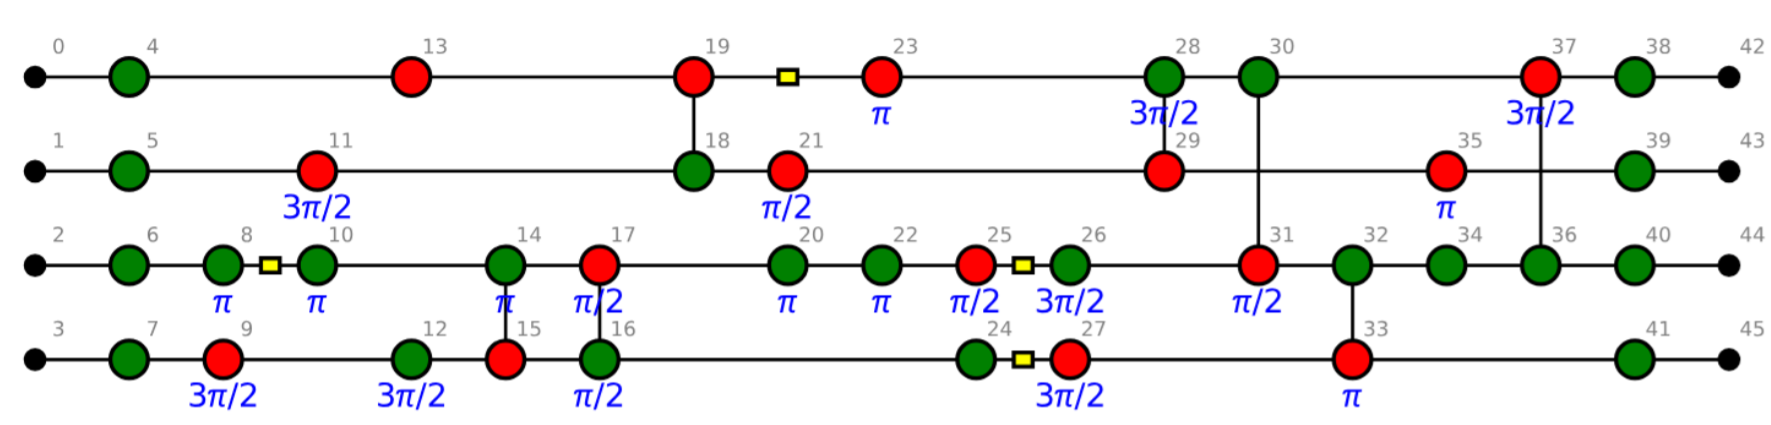
\includegraphics[width = 0.9\textwidth]{Figures/examplepyzx.png}
        \caption{Example of the default drawing method of quantum circuits.}
        \label{fig:diagram-ex}
    \end{figure}

You can also convert a circuit into a ZX-diagram:
\begin{minted}{python}
g = circuit.to_graph()
\end{minted}

To explain in further depth the simplification routines of ZX-diagrams, we will use a built-in example:
\begin{minted}{python}
zx.clifford_simp(g)  #simplifies the diagram with the clifford_simp method
g.normalize()        #makes it more presentable
zx.draw(g)
\end{minted}

\begin{figure}[ht]
        \centering
        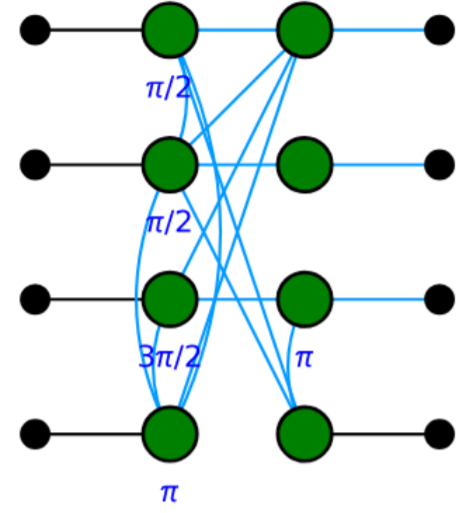
\includegraphics[scale = 0.5]{Figures/companentex.png}
        \caption{A new more compact form of the example above. The blue lines represent edges which have a Hadamard gate on them.}
        \label{fig:diagram-ex}
    \end{figure}

Internally, a ZX-diagram is represented as a \textbf{graph}.

\subsubsection{\texttt{Graph} class}
The \texttt{Graph} class is much more interesting. As you could see in the previous chapter, the graphs in PyZX are pretty simple graphs with typed vertices and edges. There are three types of vertices: boundaries, Z-spiders, and X-spiders. Every single vertex can be labelled by a phase that is stored as a fraction representing a rational multiple of $\pi$. These edges can also be divided in two types: one with a regular connection between spiders and a Hadamard-edge. 

One of the most common things to deal with PyZX graphs in ZX-Calculus is to add an edge. This can be done with the \texttt{$add\_edge$} method. However, if we add an edge where there is already one present will simply replace it. Because of this, it is sometimes more convenient to use the rules of ZX-Calculus to resolve parallel edges and self-loops whenever a new edge is added. And to use this functionality, we can use the \texttt{Graph} method \texttt{$add\_edge\_table$}, which will take in a list of edges and edge-types to then resolve how the ZX-diagram would look like when every single self-loop or double edges have been resolved. 

The \texttt{Graph} class

\section{Manually constructing an ZX-diagram}

\section{Further Resources}
As promised, we included some sources so you can deepen your knowledge in the presented information. 
